\documentclass[border=4pt]{standalone}

\usepackage{amsmath}
\usepackage{tikz}
\usepackage{mathdots}
\usepackage{yhmath}
\usepackage{cancel}
\usepackage{color}
\usepackage{siunitx}
\usepackage{array}
\usepackage{multirow}
\usepackage{amssymb}
\usepackage{gensymb}
\usepackage{tabularx}
\usepackage{booktabs}
\usetikzlibrary{fadings}
\usetikzlibrary{patterns}


\begin{document}
 

\tikzset{every picture/.style={line width=0.75pt}} %set default line width to 0.75pt        

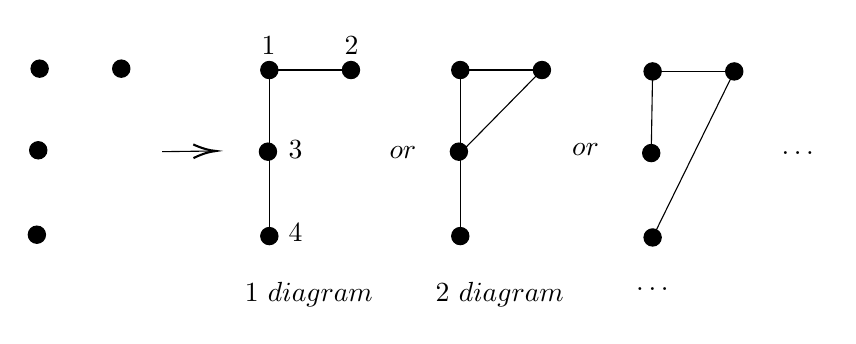
\begin{tikzpicture}[x=0.75pt,y=0.75pt,yscale=-1,xscale=1]
%uncomment if require: \path (0,300); %set diagram left start at 0, and has height of 300

%Shape: Circle [id:dp46390962399377744] 
\draw  [fill={rgb, 255:red, 0; green, 0; blue, 0 }  ,fill opacity=1 ] (37.5,81) .. controls (37.5,78.7) and (39.37,76.83) .. (41.67,76.83) .. controls (43.97,76.83) and (45.83,78.7) .. (45.83,81) .. controls (45.83,83.3) and (43.97,85.17) .. (41.67,85.17) .. controls (39.37,85.17) and (37.5,83.3) .. (37.5,81) -- cycle ;
%Shape: Circle [id:dp2796495620042718] 
\draw  [fill={rgb, 255:red, 0; green, 0; blue, 0 }  ,fill opacity=1 ] (36.83,120.33) .. controls (36.83,118.03) and (38.7,116.17) .. (41,116.17) .. controls (43.3,116.17) and (45.17,118.03) .. (45.17,120.33) .. controls (45.17,122.63) and (43.3,124.5) .. (41,124.5) .. controls (38.7,124.5) and (36.83,122.63) .. (36.83,120.33) -- cycle ;
%Shape: Circle [id:dp33848495984392724] 
\draw  [fill={rgb, 255:red, 0; green, 0; blue, 0 }  ,fill opacity=1 ] (36.17,161) .. controls (36.17,158.7) and (38.03,156.83) .. (40.33,156.83) .. controls (42.63,156.83) and (44.5,158.7) .. (44.5,161) .. controls (44.5,163.3) and (42.63,165.17) .. (40.33,165.17) .. controls (38.03,165.17) and (36.17,163.3) .. (36.17,161) -- cycle ;
%Shape: Circle [id:dp07557598820515632] 
\draw  [fill={rgb, 255:red, 0; green, 0; blue, 0 }  ,fill opacity=1 ] (76.83,81) .. controls (76.83,78.7) and (78.7,76.83) .. (81,76.83) .. controls (83.3,76.83) and (85.17,78.7) .. (85.17,81) .. controls (85.17,83.3) and (83.3,85.17) .. (81,85.17) .. controls (78.7,85.17) and (76.83,83.3) .. (76.83,81) -- cycle ;
%Straight Lines [id:da657367738113166] 
\draw    (100.67,121) -- (124.67,120.69) ;
\draw [shift={(126.67,120.67)}, rotate = 539.27] [color={rgb, 255:red, 0; green, 0; blue, 0 }  ][line width=0.75]    (10.93,-3.29) .. controls (6.95,-1.4) and (3.31,-0.3) .. (0,0) .. controls (3.31,0.3) and (6.95,1.4) .. (10.93,3.29)   ;





% Text Node
\draw (152,70) node    {$1$};
% Text Node
\draw (192,70) node    {$2$};
% Text Node
\draw (165,120) node    {$3$};
% Text Node
\draw (165,160) node    {$4$};

%Shape: Circle [id:dp90491892972551] 
\draw  [fill={rgb, 255:red, 0; green, 0; blue, 0 }  ,fill opacity=1 ] (148.17,81.67) .. controls (148.17,79.37) and (150.03,77.5) .. (152.33,77.5) .. controls (154.63,77.5) and (156.5,79.37) .. (156.5,81.67) .. controls (156.5,83.97) and (154.63,85.83) .. (152.33,85.83) .. controls (150.03,85.83) and (148.17,83.97) .. (148.17,81.67) -- cycle ;
%Shape: Circle [id:dp8943284034606729] 
\draw  [fill={rgb, 255:red, 0; green, 0; blue, 0 }  ,fill opacity=1 ] (147.5,121) .. controls (147.5,118.7) and (149.37,116.83) .. (151.67,116.83) .. controls (153.97,116.83) and (155.83,118.7) .. (155.83,121) .. controls (155.83,123.3) and (153.97,125.17) .. (151.67,125.17) .. controls (149.37,125.17) and (147.5,123.3) .. (147.5,121) -- cycle ;
%Shape: Circle [id:dp1983633427475775] 
\draw  [fill={rgb, 255:red, 0; green, 0; blue, 0 }  ,fill opacity=1 ] (148.17,161.67) .. controls (148.17,159.37) and (150.03,157.5) .. (152.33,157.5) .. controls (154.63,157.5) and (156.5,159.37) .. (156.5,161.67) .. controls (156.5,163.97) and (154.63,165.83) .. (152.33,165.83) .. controls (150.03,165.83) and (148.17,163.97) .. (148.17,161.67) -- cycle ;
%Shape: Circle [id:dp22838565266777033] 
\draw  [fill={rgb, 255:red, 0; green, 0; blue, 0 }  ,fill opacity=1 ] (187.5,81.67) .. controls (187.5,79.37) and (189.37,77.5) .. (191.67,77.5) .. controls (193.97,77.5) and (195.83,79.37) .. (195.83,81.67) .. controls (195.83,83.97) and (193.97,85.83) .. (191.67,85.83) .. controls (189.37,85.83) and (187.5,83.97) .. (187.5,81.67) -- cycle ;
%Straight Lines [id:da06808760607929654] 
\draw    (152.33,81.67) -- (191.67,81.67) ;


%Straight Lines [id:da11060601278989668] 
\draw    (152.33,81.67) -- (152.33,161.67) ;


%Shape: Circle [id:dp8665383041653496] 
\draw  [fill={rgb, 255:red, 0; green, 0; blue, 0 }  ,fill opacity=1 ] (240.17,81.67) .. controls (240.17,79.37) and (242.03,77.5) .. (244.33,77.5) .. controls (246.63,77.5) and (248.5,79.37) .. (248.5,81.67) .. controls (248.5,83.97) and (246.63,85.83) .. (244.33,85.83) .. controls (242.03,85.83) and (240.17,83.97) .. (240.17,81.67) -- cycle ;
%Shape: Circle [id:dp7088115198901408] 
\draw  [fill={rgb, 255:red, 0; green, 0; blue, 0 }  ,fill opacity=1 ] (239.5,121) .. controls (239.5,118.7) and (241.37,116.83) .. (243.67,116.83) .. controls (245.97,116.83) and (247.83,118.7) .. (247.83,121) .. controls (247.83,123.3) and (245.97,125.17) .. (243.67,125.17) .. controls (241.37,125.17) and (239.5,123.3) .. (239.5,121) -- cycle ;
%Shape: Circle [id:dp02461174937705768] 
\draw  [fill={rgb, 255:red, 0; green, 0; blue, 0 }  ,fill opacity=1 ] (240.17,161.67) .. controls (240.17,159.37) and (242.03,157.5) .. (244.33,157.5) .. controls (246.63,157.5) and (248.5,159.37) .. (248.5,161.67) .. controls (248.5,163.97) and (246.63,165.83) .. (244.33,165.83) .. controls (242.03,165.83) and (240.17,163.97) .. (240.17,161.67) -- cycle ;
%Shape: Circle [id:dp8199339523953266] 
\draw  [fill={rgb, 255:red, 0; green, 0; blue, 0 }  ,fill opacity=1 ] (279.5,81.67) .. controls (279.5,79.37) and (281.37,77.5) .. (283.67,77.5) .. controls (285.97,77.5) and (287.83,79.37) .. (287.83,81.67) .. controls (287.83,83.97) and (285.97,85.83) .. (283.67,85.83) .. controls (281.37,85.83) and (279.5,83.97) .. (279.5,81.67) -- cycle ;
%Straight Lines [id:da9018714322592571] 
\draw    (244.33,81.67) -- (283.67,81.67) ;


%Straight Lines [id:da8979385732403145] 
\draw    (244.33,81.67) -- (244.33,161.67) ;


%Shape: Circle [id:dp7716062500153196] 
\draw  [fill={rgb, 255:red, 0; green, 0; blue, 0 }  ,fill opacity=1 ] (332.83,82.33) .. controls (332.83,80.03) and (334.7,78.17) .. (337,78.17) .. controls (339.3,78.17) and (341.17,80.03) .. (341.17,82.33) .. controls (341.17,84.63) and (339.3,86.5) .. (337,86.5) .. controls (334.7,86.5) and (332.83,84.63) .. (332.83,82.33) -- cycle ;
%Shape: Circle [id:dp19022971483842066] 
\draw  [fill={rgb, 255:red, 0; green, 0; blue, 0 }  ,fill opacity=1 ] (332.17,121.67) .. controls (332.17,119.37) and (334.03,117.5) .. (336.33,117.5) .. controls (338.63,117.5) and (340.5,119.37) .. (340.5,121.67) .. controls (340.5,123.97) and (338.63,125.83) .. (336.33,125.83) .. controls (334.03,125.83) and (332.17,123.97) .. (332.17,121.67) -- cycle ;
%Shape: Circle [id:dp30290518725655624] 
\draw  [fill={rgb, 255:red, 0; green, 0; blue, 0 }  ,fill opacity=1 ] (332.83,162.33) .. controls (332.83,160.03) and (334.7,158.17) .. (337,158.17) .. controls (339.3,158.17) and (341.17,160.03) .. (341.17,162.33) .. controls (341.17,164.63) and (339.3,166.5) .. (337,166.5) .. controls (334.7,166.5) and (332.83,164.63) .. (332.83,162.33) -- cycle ;
%Shape: Circle [id:dp0906273385743972] 
\draw  [fill={rgb, 255:red, 0; green, 0; blue, 0 }  ,fill opacity=1 ] (372.17,82.33) .. controls (372.17,80.03) and (374.03,78.17) .. (376.33,78.17) .. controls (378.63,78.17) and (380.5,80.03) .. (380.5,82.33) .. controls (380.5,84.63) and (378.63,86.5) .. (376.33,86.5) .. controls (374.03,86.5) and (372.17,84.63) .. (372.17,82.33) -- cycle ;
%Straight Lines [id:da36394006735961937] 
\draw    (337,82.33) -- (376.33,82.33) ;


%Straight Lines [id:da4684133478442791] 
\draw    (376.33,82.33) -- (337,162.33) ;


%Straight Lines [id:da05740445391425775] 
\draw    (283.67,81.67) -- (244.33,121.67) ;


%Straight Lines [id:da7303970440355139] 
\draw    (337,82.33) -- (336.33,121.67) ;



% Text Node
\draw (216.67,121.33) node    {$or$};
% Text Node
\draw (408,121.67) node    {$\dotsc $};
% Text Node
\draw (304.67,120) node    {$or$};
% Text Node
\draw (171.33,189.67) node    {$1\ diagram$};
% Text Node
\draw (263.33,189.67) node    {$2\ diagram$};
% Text Node
\draw (338,187) node    {$\dotsc $};


\end{tikzpicture}
\end{document}
